\documentclass[11pt]{article}

\usepackage[margin=1in]{geometry}
\usepackage{amsmath,amssymb}
\usepackage{booktabs}
\usepackage{graphicx}
\usepackage{microtype}
\usepackage[numbers,sort&compress]{natbib}
\usepackage[hidelinks]{hyperref}

\emergencystretch=2em

\graphicspath{{figures/}}

\title{Testing Role-Specific Corrections for Tied Input and Output Embeddings}
\author{Arjun Shah}
\date{September 2026}

\begin{document}
\newcommand{\PrimarySeedCount}{3}
\newcommand{\TiedFinalLoss}{5.06856}
\newcommand{\PartialFinalLoss}{5.10784}
\newcommand{\UntiedFinalLoss}{5.42733}
\newcommand{\CapacityFinalLoss}{5.27932}
\newcommand{\TiedFinalPPL}{158.95}
\newcommand{\PartialFinalPPL}{165.33}
\newcommand{\UntiedFinalPPL}{227.64}
\newcommand{\PartialExtraParams}{810{,}256}
\newcommand{\UntiedExtraParams}{19{,}298{,}688}
\newcommand{\CapacityExtraParams}{811{,}008}
\newcommand{\PartialVsTiedDelta}{0.03928}
\newcommand{\UntiedVsTiedDelta}{0.35877}
\newcommand{\CapacityVsTiedDelta}{0.21076}
\newcommand{\RecoveryStatus}{untied\ not\ better\ than\ tied}

\maketitle

\begin{abstract}
Weight tying uses one vocabulary matrix both to embed input tokens and to score output tokens. We test whether a shared base plus small role-specific low-rank corrections can retain the parameter savings of tying while recovering flexibility from untying. The main study uses a six-layer decoder-only Transformer on WikiText-2-raw-v1, three seeds, and 50,000 fresh optimizer steps. The tied model reaches final validation loss \TiedFinalLoss, compared with \PartialFinalLoss for rank-8 partial tying and \UntiedFinalLoss for full untying. The paired partial-minus-tied difference is +\PartialVsTiedDelta, while untied-minus-tied is +\UntiedVsTiedDelta; lower is better. Because full untying is worse than tying, an untied-benefit recovery fraction is undefined. A three-seed rank replication, a parameter-matched control, a smaller model, Tiny Shakespeare, path interventions, and representation probes do not reveal a stable partial-tying quality advantage. The evidence supports a narrow negative and mechanistic conclusion: in these small-model regimes, tied embeddings are a strong baseline, role-specific corrections move measurably, and that movement does not improve language-modeling loss.
\end{abstract}

\section{Introduction}

Decoder-only language models commonly use weight tying: the matrix that maps token IDs to vectors is also transposed to produce vocabulary logits. This saves a vocabulary-sized matrix and often works well, but the input and output pathways receive different signals. The input pathway represents token identities for the Transformer; the output pathway ranks the next-token vocabulary from a contextual hidden state.

We study a middle ground rather than assuming that either exact equality or complete independence is correct. Let $W_{\mathrm{shared}}\in\mathbb{R}^{V\times D}$ be a shared base. The partial model uses
\begin{equation}
 W_{\mathrm{input}} = W_{\mathrm{shared}} + s A_{\mathrm{input}}B_{\mathrm{input}}^\top,
 \qquad
 W_{\mathrm{output}} = W_{\mathrm{shared}} + s A_{\mathrm{output}}B_{\mathrm{output}}^\top,
\end{equation}
where $A\in\mathbb{R}^{V\times r}$, $B\in\mathbb{R}^{D\times r}$, and $s=\alpha/r$. The extra parameter cost is $2r(V+D)$, much smaller than adding a second full vocabulary matrix when $r\ll D$.

The central empirical question is how much of an untied quality benefit can such corrections recover per added parameter. We compare tied, fully untied, rank-8 partial, and a parameter-matched tied control under identical Transformer, optimizer, data, seed, validation, and token-exposure conditions. The paper follows the evidence even when the untied baseline is not better than tied.

\begin{figure}[t]
\centering
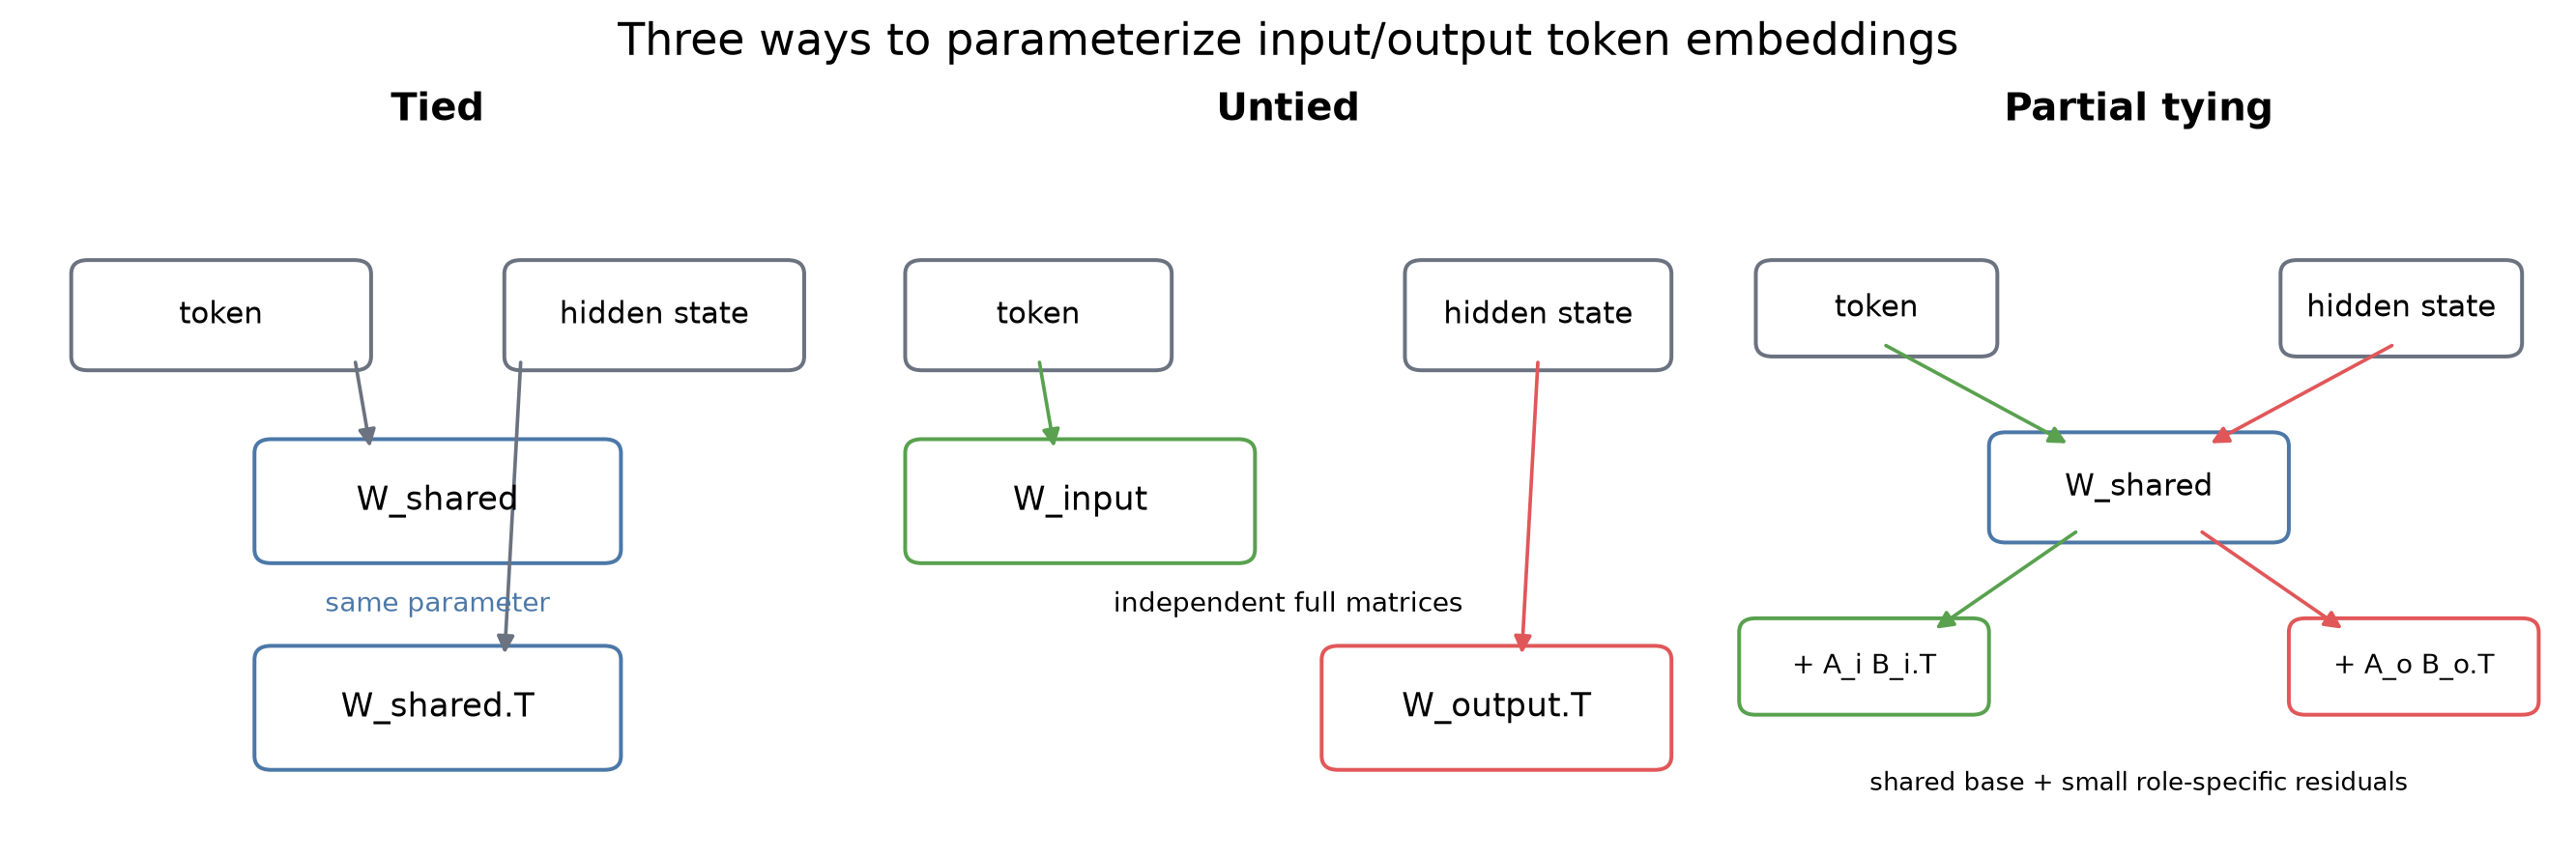
\includegraphics[width=\linewidth]{architecture.png}
\caption{Tied, untied, and partially tied input/output parameterizations.}
\label{fig:architecture}
\end{figure}

\section{Related work}

Weight tying was introduced as a practical and theoretically motivated parameter-sharing method by Press and Wolf and by Inan, Khosravi, and Socher \citep{press2017using,inan2017tying}. Press and Wolf also reported that the tied representation evolves more like the output embedding than the untied input embedding, motivating pathway-specific diagnostics. Work on the geometry and role distinction of input and output representations includes Gulordava, Aina, and Boleda and Derby, Miller, and Devereux \citep{gulordava2018represent,derby2020analysing}.

Several methods relax the hard equality constraint. Chung et al. study decoupled input and output embedding dimensions in pretrained language models \citep{chung2021rethinking}. Adaptive input representations allocate variable capacity across vocabulary regions \citep{baevski2019adaptive}; that goal differs from our role-specific residuals on a shared full-width base. Low-rank adaptation supplies the factorized parameterization used here \citep{hu2022lora}.

More recent work connects tying to distributional assumptions and possible output-space bias \citep{bertolotti2024tying,lopardo2026weight}, while other alternatives change the shared interface or use a compact input representation with a separate output head \citep{batley2026separable,gu2026pseudoinverse}. Rather than choosing between fully tied and fully untied embeddings, this project studies whether a large shared base plus small role-specific low-rank residuals can recover flexibility at a fraction of the parameter cost. The contribution is a controlled empirical comparison and measurement pipeline, not a claim of broad architectural novelty.

\section{Method and fair comparison}

All conditions use the same decoder-only Transformer. The primary configuration has six layers, six attention heads, width 384, context length 256, GPT-2 BPE tokenization, and WikiText-2-raw-v1. The main 50k study uses seeds 1337, 2027, and 31415, batch size 2, 50,000 fresh optimizer steps, warmup 100, and cosine decay from $3\times10^{-4}$ to $3\times10^{-5}$. Every condition within a seed receives the same sampled training windows, optimizer schedule, fixed validation windows, initialization protocol, and token budget.

The tied model uses one parameter for lookup and projection. The untied model copies the tied initialization into independent input and output parameters. The partial model starts with zero effective corrections and therefore the same initial function as tied. The capacity control adds approximately the partial model's parameter budget elsewhere in the Transformer without separating input and output roles. Study 1 additionally includes input-only and output-only corrections.

The optimized partial computation never constructs a full correction matrix during normal training. Input lookup is
\[
W_{\mathrm{shared}}[x] + s A_{\mathrm{input}}[x]B_{\mathrm{input}}^\top,
\]
and output projection is
\[
hW_{\mathrm{shared}}^\top + s(hB_{\mathrm{output}})A_{\mathrm{output}}^\top.
\]
Tests compare these operations with explicit small-matrix reconstruction. Full matrices are used only for analysis diagnostics.

The validator requires a complete seed-by-condition matrix, matching configurations and pinned dataset hashes, finite metrics, a validation record exactly at the declared final step, and exact equality of actual token exposure and sampled-offset digests. All confidence intervals below are deterministic bootstrap intervals over paired seeds and are descriptive at $n=3$.

\section{Main result}

Table~\ref{tab:primary} reports the fresh 50k study. Tied has the lowest final and best validation losses. Rank-8 partial adds \PartialExtraParams{} parameters, about 2.7\% of the tied model, while full untying adds \UntiedExtraParams{}, about 64.3\% of the tied model. Partial is substantially cheaper than untied, but its final loss is higher than tied by a positive paired difference. Since untied is also higher than tied, the usual recovered-fraction statistic is not meaningful here.

\begin{table}[t]
\centering
\caption{Fresh 50k primary study. Values are means across three seeds; intervals in the table are bootstrap intervals for final loss.}
\label{tab:primary}
\resizebox{\linewidth}{!}{\begin{tabular}{lrrrrrr}
\toprule
Condition & Params. & $\Delta$ params. & Final loss & 95\% CI & Best loss & Seeds \\
\midrule
capacity\_control & 30{,}834{,}816 & 811{,}008 & 5.36654 & [5.3488, 5.3903] & 5.36654 & 3 \\
partial & 30{,}834{,}064 & 810{,}256 & 5.37736 & [5.3461, 5.4012] & 5.37700 & 3 \\
partial\_input & 30{,}428{,}936 & 405{,}128 & 5.38157 & [5.3565, 5.4045] & 5.38114 & 3 \\
partial\_output & 30{,}428{,}936 & 405{,}128 & 5.37348 & [5.3401, 5.4030] & 5.37348 & 3 \\
tied & 30{,}023{,}808 & 0 & 5.37413 & [5.3516, 5.3942] & 5.37382 & 3 \\
untied & 49{,}322{,}496 & 19{,}298{,}688 & 5.43876 & [5.4083, 5.4626] & 5.43827 & 3 \\
\bottomrule
\end{tabular}
}
\end{table}

\begin{figure}[t]
\centering
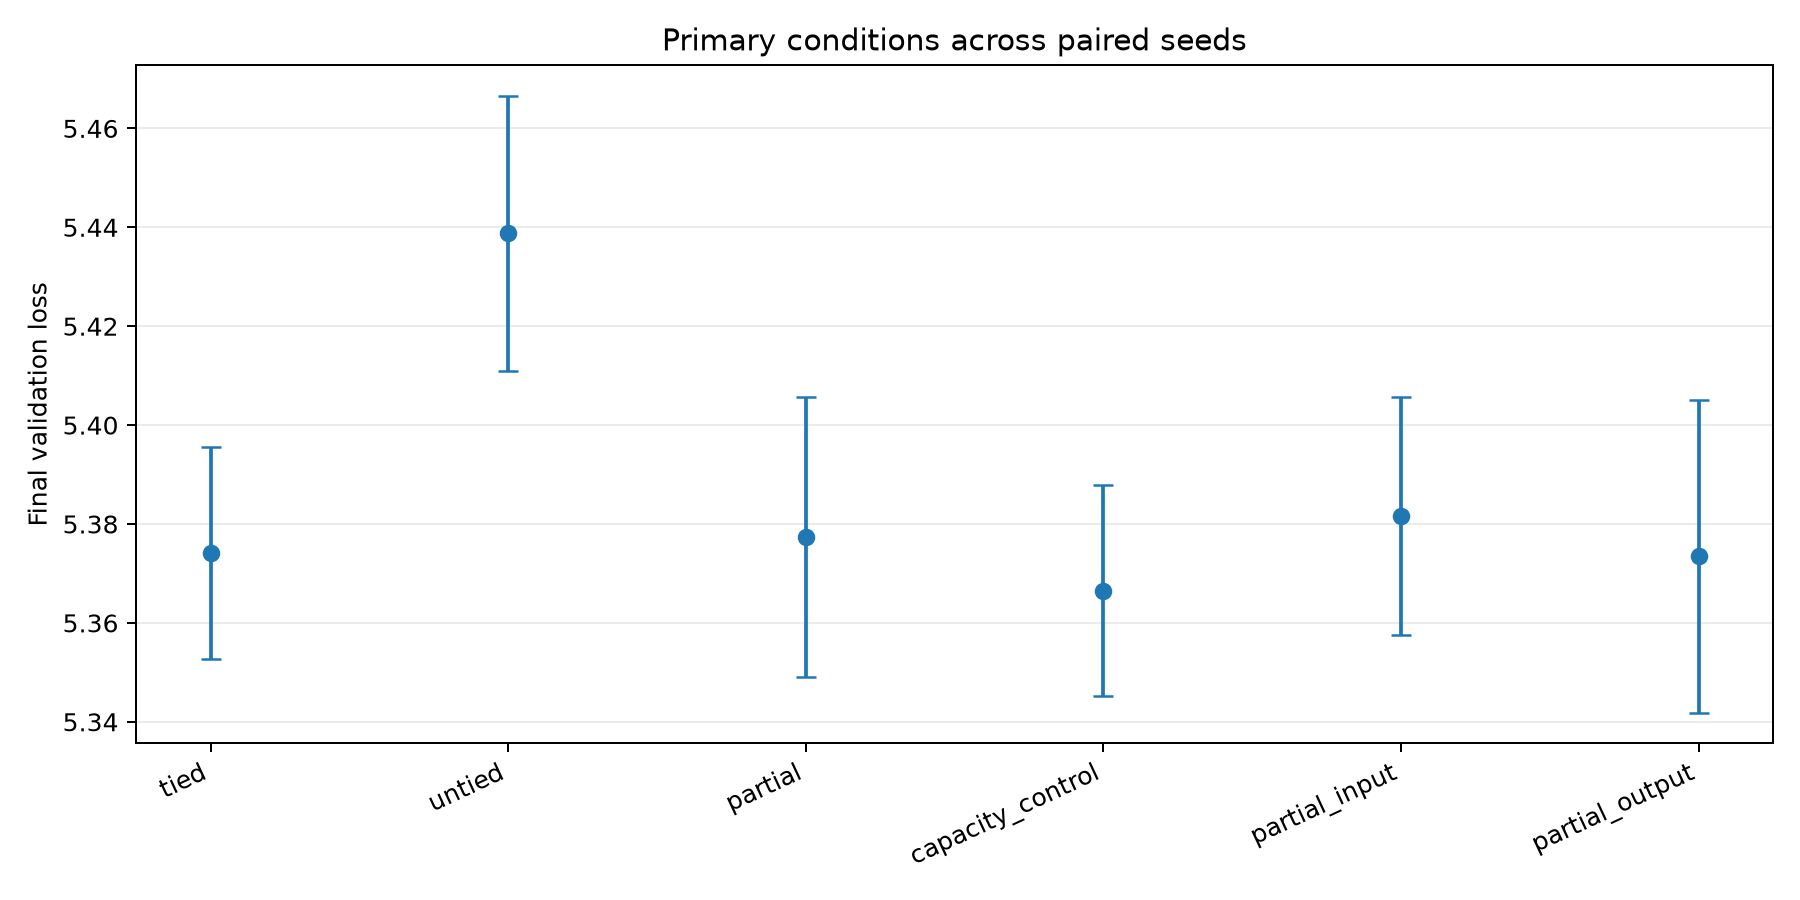
\includegraphics[width=0.48\linewidth]{final_loss_by_condition.png}
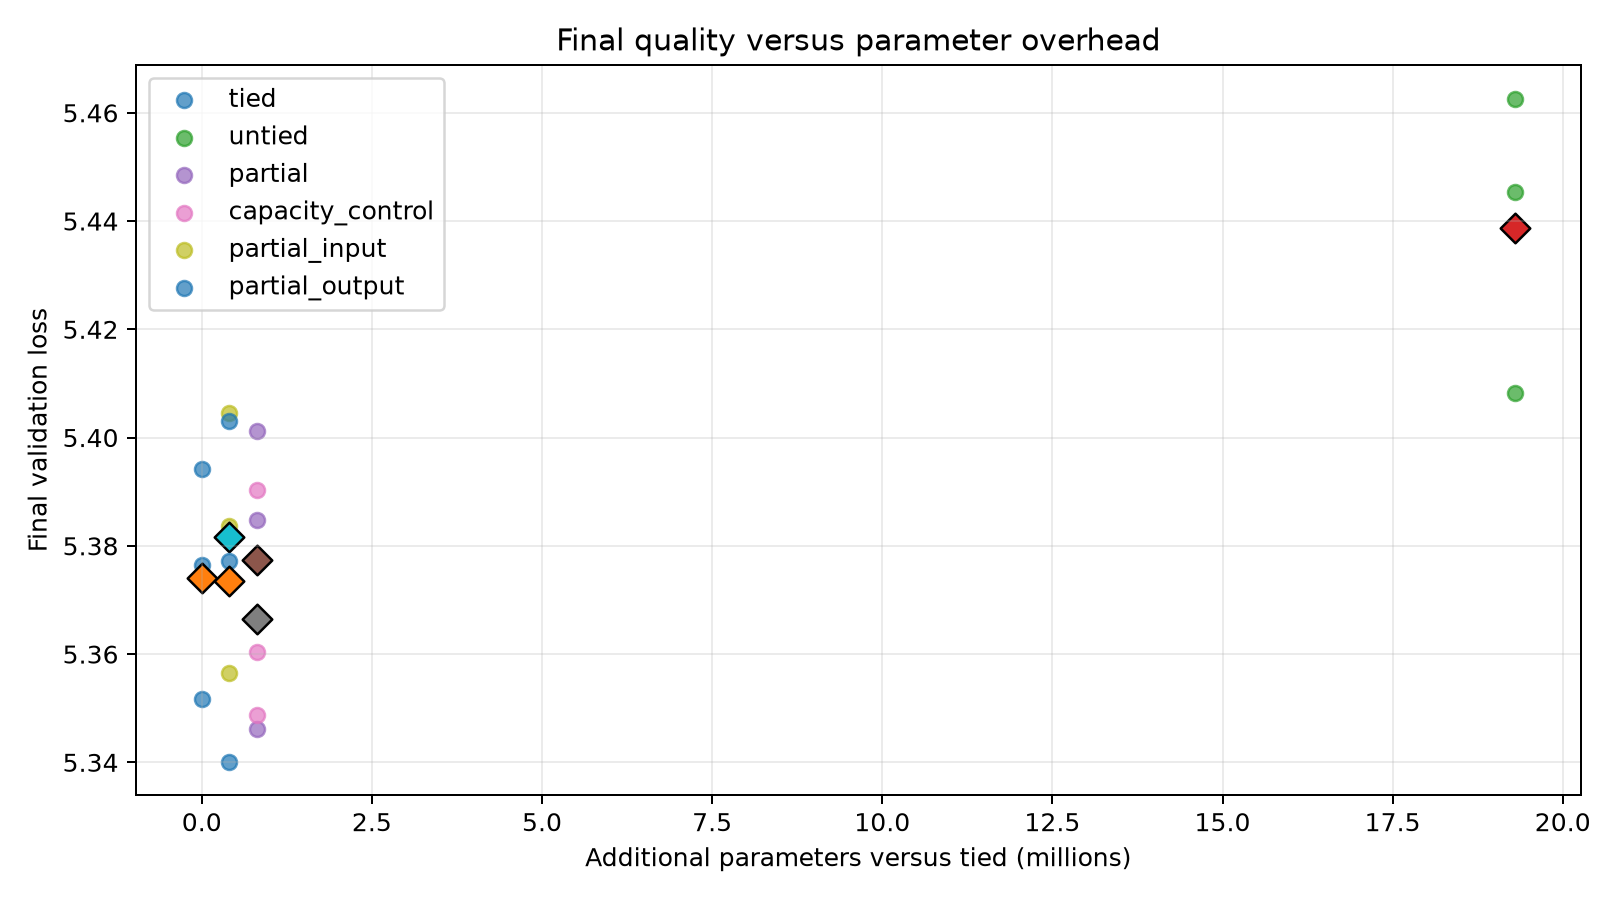
\includegraphics[width=0.48\linewidth]{parameter_efficiency.png}
\caption{Final loss and parameter-efficiency views of the fresh 50k primary study.}
\label{fig:primary}
\end{figure}

The parameter-matched tied control has nearly the same parameter count as partial but a worse final loss. This separates the role-specific comparison from the claim that any additional capacity must help. The control is not compute-matched: its width increase changes Transformer FLOPs, and the partial model adds factorized projection work. We therefore report parameters, estimated FLOPs, throughput, and memory separately rather than collapsing them into one score.

\section{Rank replication and robustness}

The 10k rank replication uses ranks 1, 2, 4, 8, 16, and 32 with the same three seeds and a frozen protocol. Table~\ref{tab:rank} reports paired final-loss differences against tied. Every mean difference is nonnegative. Rank 32 is closest in mean, but its interval crosses zero, and no rank provides a stable improvement. The rank sweep therefore does not justify selecting rank 8, rank 16, or any other rank as a winning setting.

\begin{table}[t]
\centering
\caption{Three-seed 10k rank replication. Paired differences are partial rank minus tied; lower loss is better.}
\label{tab:rank}
\resizebox{\linewidth}{!}{\begin{tabular}{rrrrrr}
\toprule
Rank & Extra params. & Final loss & Paired $\Delta$ & Descriptive bootstrap interval & Seeds \\
\midrule
1 & 101{,}282 & 5.37634 & 0.0022 & [-0.0111, 0.0098] & 3 \\
2 & 202{,}564 & 5.38376 & 0.0096 & [0.0051, 0.0179] & 3 \\
4 & 405{,}128 & 5.37741 & 0.0033 & [-0.0014, 0.0108] & 3 \\
8 & 810{,}256 & 5.37736 & 0.0032 & [-0.0056, 0.0083] & 3 \\
16 & 1{,}620{,}512 & 5.37819 & 0.0041 & [-0.0162, 0.0255] & 3 \\
32 & 3{,}241{,}024 & 5.37613 & 0.0020 & [-0.0067, 0.0089] & 3 \\
\bottomrule
\end{tabular}
}
\end{table}

\begin{figure}[t]
\centering
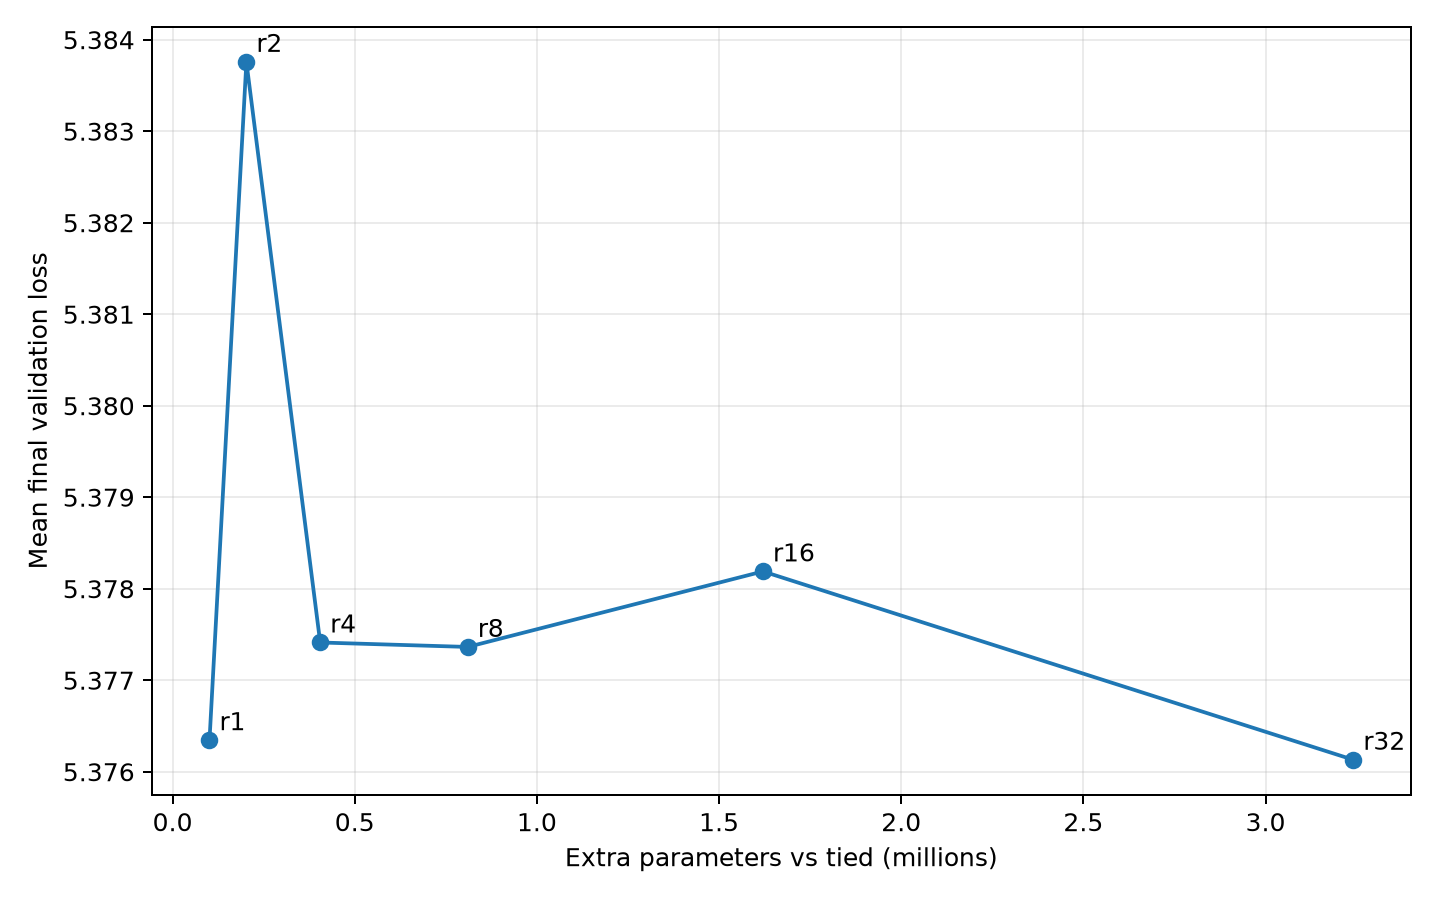
\includegraphics[width=0.48\linewidth]{rank_vs_extra_parameters.png}
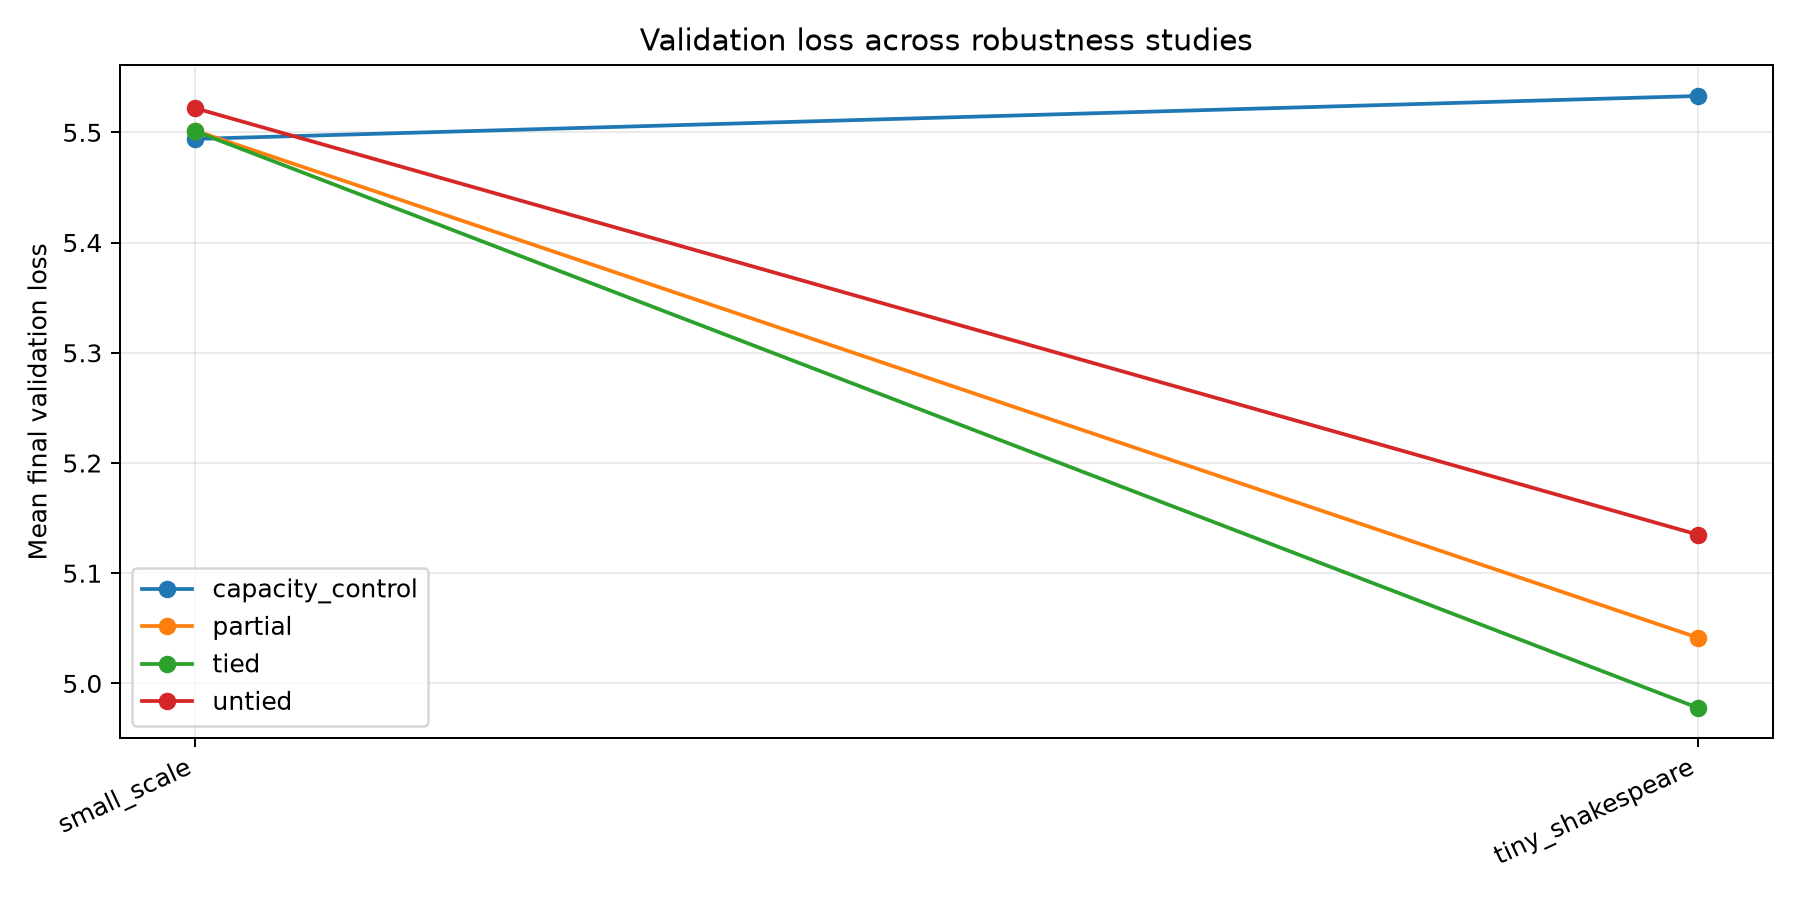
\includegraphics[width=0.48\linewidth]{robustness_final_loss.png}
\caption{Rank/parameter tradeoff and mean final loss in the two robustness studies.}
\label{fig:robustness}
\end{figure}

The robustness studies repeat the central comparison with three seeds at a smaller WikiText-2 model and on Tiny Shakespeare. The smaller model gives tied 5.50110, partial 5.50163, and untied 5.52198 final loss; the partial-minus-tied paired difference is uncertain. Tiny Shakespeare gives tied 4.97787, partial 5.04152, and untied 5.13499. The final-checkpoint result does not show a partial gain, and the Tiny Shakespeare capacity control exhibits late overfitting. These studies do not establish a universal ordering, but they do not rescue the original partial-tying hypothesis.

\begin{table}[t]
\centering
\caption{Selected robustness endpoints generated from the secondary aggregate.}
\label{tab:secondary}
\resizebox{\linewidth}{!}{\begin{tabular}{llrrrr}
\toprule
Study & Condition & Params. & Extra & Final loss & Seeds \\\\
\midrule
small\_scale & capacity\_control & 16{,}890{,}112 & 808{,}448 & 5.49405 & 3 \\
small\_scale & partial & 16{,}889{,}872 & 808{,}208 & 5.50163 & 3 \\
small\_scale & tied & 16{,}081{,}664 & 0 & 5.50110 & 3 \\
small\_scale & untied & 28{,}947{,}456 & 12{,}865{,}792 & 5.52198 & 3 \\
tiny\_shakespeare & capacity\_control & 30{,}834{,}816 & 811{,}008 & 5.53302 & 3 \\
tiny\_shakespeare & partial & 30{,}834{,}064 & 810{,}256 & 5.04152 & 3 \\
tiny\_shakespeare & tied & 30{,}023{,}808 & 0 & 4.97787 & 3 \\
tiny\_shakespeare & untied & 49{,}322{,}496 & 19{,}298{,}688 & 5.13499 & 3 \\
\bottomrule
\end{tabular}
}
\end{table}

\section{Mechanism measurements}

The training code decomposes input-path and output-path pressure in effective $V\times D$ embedding-matrix space. This avoids treating gradients of the low-rank factors as if their arbitrary bases were scientifically meaningful. We record the total and shared-matrix gradient norms, output/input ratios, effective gradient cosines, cumulative update path, correction norms, effective ranks, singular spectra, correction alignment, token classes, and matched-frequency buckets.

At the final 50k measurement, the tied output/input ratio is approximately 1.00 and the rank-8 partial ratio is approximately 0.97. The effective gradient cosine is close to zero for both. The partial output correction is larger in norm than its input correction, and both corrections use their available rank, but input/output correction alignment remains weak. These observations show role-specific movement without showing that the movement is useful for language modeling.

The matched three-seed path interventions stop input or output gradients for steps $[0,5000)$. Stopping input gradients changes partial minus tied final loss by +0.00037 with a 95\% interval $[-0.00676,+0.00798]$. Stopping output gradients changes it by -0.00618 with interval $[-0.01474,+0.01011]$. Neither is a stable paired causal effect at this sample size.

\begin{table}[t]
\centering
\caption{Final effective gradient and correction diagnostics from the 50k primary study.}
\label{tab:mechanism}
\resizebox{\linewidth}{!}{\begin{tabular}{lrrrrr}
\toprule
Condition & Out./in. grad. & Grad. cosine & Input $\Delta_i$ norm & Output $\Delta_o$ norm & $\Delta_i$/$\Delta_o$ cosine \\
\midrule
Tied & 1.0044 & 0.0017 & 0.0000 & 0.0000 & 0.0000 \\
Partial & 0.9733 & 0.0014 & 14.9951 & 93.4143 & -0.0040 \\
Capacity control & 1.4464 & 0.0086 & 0.0000 & 0.0000 & 0.0000 \\
\bottomrule
\end{tabular}
}
\end{table}

\begin{table}[t]
\centering
\caption{Three-seed path-intervention effects at 10k. Each value is partial minus tied final validation loss.}
\label{tab:interventions}
\begin{tabular}{lrrr}
\toprule
Stopped path & Paired final $\Delta$ & Descriptive bootstrap interval & Seeds \\
\midrule
Input & 0.00037 & [-0.0068, 0.0080] & 3 \\
Output & -0.00618 & [-0.0147, 0.0101] & 3 \\
\bottomrule
\end{tabular}

\end{table}

\section{Representation evaluation}

Language-modeling loss is not treated as a direct measure of input embedding quality. The completed runs include frequency-matched nearest-neighbor cosine and agreement, lexical pair scores, and frozen linear probes for token metadata. In the 50k WikiText-2 evaluation, tied has mean input nearest-neighbor cosine 0.659 and frequency-matched agreement 0.481; partial has 0.647 and 0.482. The two models are close on these diagnostics, while untied is lower on both. The probe results do not provide evidence that partial corrections improve input representations in this setting. Output-side evaluation remains separate from input-side evaluation.

\section{Limitations}

The main study uses one tokenizer, one WikiText-2 configuration, and three seeds. The rank replication is 10k rather than 50k, and the robustness studies use a smaller model and Tiny Shakespeare rather than a large corpus or a modern large-language-model scale. Three seeds give useful paired estimates but wide limits on subtle effects. FLOP counts are estimates based on declared dense and factorized operations, not hardware-independent measurements. The representation probes are frozen token-level diagnostics, not downstream task evaluations. The findings should therefore be read as a careful result for the tested regime, not as a claim about all embedding architectures or language models.

\section{Reproducibility}

The release includes the source commits used for each study, pinned dataset hashes, the frozen environment, Kaggle launch and collection tooling, per-run configuration and metrics, batch-stream digests, fairness outputs, aggregate JSON, plots, generated tables, and an independently compilable arXiv bundle. Large checkpoints, optimizer states, and downloaded corpora are excluded. The 10k Study 1 artifacts remain available as a separate preliminary endpoint and are never mixed into the 50k primary aggregate.

\section{Conclusion}

This study asked whether a shared vocabulary matrix with small role-specific low-rank corrections could recover a useful benefit from untied input/output embeddings at much lower parameter cost. In the tested regime, the answer is no. Tied embeddings are the strongest primary model, full untying is substantially worse, and rank-8 partial tying is cheaper but also worse than tied. Rank replication and robustness checks do not reveal a stable partial advantage. Mechanism diagnostics show that role-specific gradients and corrections exist, but the measured specialization is not sufficient to improve validation loss. This narrows the useful claim: asymmetric optimization pressure can be present without creating a quality/parameter Pareto improvement from low-rank role corrections.

\bibliographystyle{plainnat}
\bibliography{references}

\end{document}
